\documentclass{llncs}

\usepackage{amsmath}
\usepackage{amssymb}
\usepackage{cancel}
\usepackage{allrunes}
\usepackage{graphics}
\usepackage{verbatim}
\usepackage{color}
\usepackage{tikz}
\usepackage[curve]{xypic}
\usetikzlibrary{arrows}
\usepackage{algorithm2e}
\usepackage{fontenc}

\graphicspath{{./img/}}

\newcommand{\argref}{\Sigma}
\newcommand{\canon}{E_\phi^{M_\mu}}
\newcommand{\canonp}{E_\phi^{M'_\mu}}
\newcommand{\restr}[2]{{#1}|_{#2}}
\newcommand{\afs}[1]{\longrightarrow(#1)}
\newcommand{\three}{\{1,0,\hf\}}
\newcommand{\prl}{\vdash_{\L}}
\newcommand{\prb}{\vdash_{\cdia}}
\newcommand{\mm}{\mathcal M}
\newcommand{\agents}{\mathcal A}
\newcommand{\lang}{\mathcal L}
\newcommand{\langa}{\lang_1}
\newcommand{\langb}{\lang_2}
\newcommand{\langl}{\lang^{\tiny {\L}}}
\newcommand{\lblack}{\lang^{\cdia}}
\newcommand{\lwhite}{\lang^{\lozenge}}
\newcommand{\lctl}{\lang^{CTL}}
\newcommand{\black}{{\bf BLACK}}
\newcommand{\hf}{\frac 12}
\newcommand{\graph}{\Pi\times\Pi}
\newcommand{\graphs}{2^{(\graph)}}
\newcommand{\model}[1]{\models_{#1}}
\newcommand{\modluk}{\models_{\tiny\L}}
\newcommand{\ddia}[1]{\langle{#1}\rangle}
\newcommand{\dbox}[1]{[#1]}
\newcommand{\adia}{\lozenge}
\newcommand{\adiastar}{\lozenge^*}
\newcommand{\abox}{\square}
\newcommand{\cdia}{\blacklozenge}
\newcommand{\cbox}{\blacksquare}
\newcommand{\lad}{\langle\leftarrow\rangle}
\newcommand{\rad}{\langle\rightarrow\rangle}
\newcommand{\lab}[2]{\Pi_{#1}(#2)}
\newcommand{\ist}{{\bf L}}
\newcommand{\notf}{{\bf M}}
\newcommand{\und}{{\bf U}}
\newcommand{\ov}[1]{\overline {#1}}
\newcommand{\ovto}[1]{\overline {\ov #1}}
\newcommand{\acro}[1]{\textsc{#1}}

\newcommand{\anext}{\mathbf{A}\bigcirc}
\newcommand{\auntil}[1]{\mathbf{A}\,{#1}\,\mathcal{U}\,}
\newcommand{\euntil}[1]{\mathbf{E}\,{#1}\,\mathcal{U}\,}

%% OK. TAR DE MED SELV OM DE ER UN0DVENDIGE! 
\newcommand{\band}{\bigwedge}
\newcommand{\bor}{\bigvee}



\newcommand{\truls}[1]{\textcolor{magenta}{(truls: #1)}}
\newcommand{\sjur}[1]{\textcolor{cyan}{(sjur: #1)}}


\newcommand{\cl}{cl}
\newcommand{\witness}[1]{{\sf w^{#1}}}
\newcommand{\buffer}[2]{{\sf b}_{#1}(#2)}
\newcommand{\sdepth}[2]{d_{#1}(#2)}
\newcommand{\shrink}[2]{\rho_{#1}(#2)}
\newcommand{\comp}[2]{C(#1,#2)}
\newcommand{\test}[1]{{#1}?}
\newcommand{\dlangm}{{\mathcal L}_{\acro{DDL}}^{-}}
\newcommand{\pis}[1]{{\mathbf e}_{#1}}
\newcommand{\carriers}[1]{Q_{#1}}
\newcommand{\kmod}[2]{{\cal K}_{(#1,#2)}}
\newcommand{\rels}[1]{{\sf R_{#1}}}
\newcommand{\update}[3]{{\mathcal U}_{#1}(#2,#3)}
\newcommand{\cons}[1]{{\textara{\ea}}(#1)}
\newcommand{\af}{(S, E)}
\newcommand{\afn}{S}
\newcommand{\afe}{E}
\newcommand{\seq}[1]{\overrightarrow{#1}}
\newcommand{\basis}{basis }
\newcommand{\state}{state }
\newcommand{\views}{\mathcal B}
\newcommand{\viewsv}{\left(V_a\right)_{(a \in \agents)}}
\newcommand{\carrier}{Q_\views}
\newcommand{\sem}{\varepsilon}
\newcommand{\depth}[1]{|{#1}|^\adia}
\newcommand{\bisim}{\underline{\leftrightarrow}}

\title{Computing consensus: A logic for reasoning about deliberative processes based on argumentation}
\author{S \& T}

\begin{document}

\maketitle

\begin{abstract}
We consider multi-agent argumentation, where each agent's view of the arguments is encoded as an AF. Then we study deliberative processes than can occur on this basis. We think of a deliberative process as taking the shape of a step-wise aggregation of a single joint AF, and we are interested in reasoning about the space of possible outcomes, provided the deliberative process satisfies \emph{faithfulness}, a postulate amounting to requiring that whenever deliberation leads to a new relationship being introduced between two arguments, this relationship is endorsed by at least on participating agent. We use the language of propositional dynamic logic to reason about the resulting deliberative structures, and we provide some technical results on model checking and reachability, demonstrating that the resulting logic is computationally well-behaved as long as agent's AFs are finitely branching.
\end{abstract}

\section{Introduction}\label{sec:intro}

\section{Background on abstract argumentation}\label{sec:abt}

Given a digraph $\af = (S,E)$, we inherit the notion of an extension from argumentation theory. With respect to some semantic $\sem$ we always have some map, mapping from $q$ to the set of acceptable arguments. We do not specify the semantic, but require that it satisfies certain properties.

\begin{definition} Let $\sem$ be a (argumentation theory) semantic, and $q \in \carriers \views$. 
\begin{itemize}
\item Elements of $\sem(q)$ partition the set of arguments into three partitions. That is, $\sem(q) \subseteq 3^\Pi$. 
\end{itemize}
\end{definition}

We make very weak assumptions about the nature of $\sem$, but we need a few assumptions and some terminology. If $\pi \in \sem(q)$, $\pi$ partitions the set of arguments into three partitions. We will refer to these as $(\pi_1, \pi_0, \pi_\hf)$. The intended interpretation of this partitioning is that we consider the set $\pi_1$ as accepted, $\pi_0$ as defeated, and $\pi_\hf$ as \emph{undecided}. We make some assumption about $\sem$: \truls{Verify!}
\begin{description}
\item[Conflict-freeness] If $\pi \in \sem(q)$, then $(\pi_1)^2 \cap q_E = \emptyset$.
\item[Defeating] Arguments $\pi_1$ defeats arguments they attack. If $\pi \in \sem(q)$, for every $y \in \pi_0$, there is an $x \in \pi_1$ such that $(x,y) \in q_E$.
\item[Undecided is not defeated] $\pi_1 \times \pi_\hf \cap q_E = \emptyset$
\item[Local interaction] Membership in $\pi_1$ is dependent only on the connected component in which the atom occurs. 
\end{description}

$$ \alpha \quad ::= \quad p ~|~ \neg \alpha ~|~ \alpha \to \alpha $$
where $p \in \Pi$.

The satisfaction relation for this logic must also satisfy certain properties. 

\begin{definition}[$\alpha$-satisfaction] Let $q \in \carriers \views$ and $\pi \in \sem(q)$, we extend the the partitioning to also interpret more complex $\alpha$-formulas as defined inductively by
\begin{align*}
\overline\pi(p) &= \pi(p) \\
\overline\pi(\neg\alpha) &= 1 - \overline\pi(\alpha)\\
\overline\pi(\alpha_1 \to \alpha_2) &= \min \{1, 1 - ((1 - \overline\pi(\alpha_1)) - \overline\pi(\alpha_2))\} 
\end{align*}
\end{definition}
It can be seen that this extension is consistent with the requirements we outlined above. \truls{ref. \& check?}

\section{Deliberative dynamic logic}\label{sec:ddl}

In this section we introduce Deliberative dynamic logic (\acro{ddl}), using the language of \acro{pdl} to reason about deliberative structures that encode step-wise deliberation. 

We assume given a set $\agents$ of agents and a countably infinite set $\Pi$ of arguments.\footnote{Possibly "statements" or "positions", depending on the context of application. \sjur{I will provide some references for that}} The basic building block of dynamic deliberative logic is provided in the following definition.

\begin{definition}\label{def:basis} A \basis for deliberation is an $\agents$-indexed collection of digraphs $\views = (V_a)_{(a \in \agents)}$, such that for each $a \in \agents$, $V_a \subseteq \Pi \times \Pi$.
\end{definition}

Given a basis which encodes agents' view of the arguments, we are interested in the possible ways in which agents can deliberate to reach \emph{agreement} on how arguments are related. That is, we are interested in the set of all AFs that can plausibly be seen as resulting from a \emph{consensus} regarding the status of the arguments in $\Pi$. What restrictions is it reasonable to place on a consensus? It seems that while many restrictions might arise from pragmatic considerations, and be implemented by specific protocols for "good" deliberation in specific contexts, there are few restrictions that can be regarded as completely general. For instance, while there is often good reason to think that the position held by the majority will be part of a consensus, it is hardly possible to stipulate an axiomatic restriction on the notion of consensus amounting to the principle of majority rule. Indeed, sometimes deliberation takes place and leads to a single dissenting voice convincing all the others, and often, these deliberative processes are far more interesting than those that transpire along more conventional lines. However, it seems reasonable to assume that whenever \emph{all} agents agree on how an argument $p$ is related to an argument $q$, then this relationship is part of any consensus. This, indeed, is the only restriction we will place on the notion of a consensus; that when the AF $\af$ is a consensus for $\basis$, it must satisfy the following \emph{faithfulness} requirement.
\begin{itemize}
\item \emph{For all $p,q \in \Pi$, if there is no disagreement about $p$'s relationship to $q$ (attack/not attack), then this relationship is part of $\af$}
\end{itemize}

This leads to the following definition of the set $\cons \views$, which we will call the set of \emph{complete assents} for $\views$, collecting all AFs that are faithful to $\views$.

\begin{equation}\label{def:consensus}
\cons \views = \left\{\af \subseteq \Pi \times \Pi ~\left|~ \bigcap_{a \in \agents}V_a \subseteq \af \bigcup_{a \in \agents}V_a \right.\right\}
\end{equation}

An element of $\cons \views$ represents a possible consensus among agents in $\agents$, but it is an \emph{idealization} of the notion of assent, since it disregards the fact that in practice, assent tends to be \emph{partial}, since it results from a dynamic process, emerging through \emph{deliberation}. Indeed, unless there is some upper bound on the number of arguments that can be introduced in a deliberative scenario we can \emph{never} hope to arrive at complete assent via deliberation. We can, however, initiate a process by which we reach agreement on more and more arguments, in the hope that this will approximate some complete assent, or maybe even be \emph{robust}, in the sense that there is \emph{no} deliberative future where the results of current partial agreement end up being undermined.

When and how deliberation might successfully lead to an approximation of complete assent is a question well suited to investigation with the help of dynamic logic. The dynamic element will be encoded using a notion of a deliberative event -- centered on an argument -- such that the set of ways in which to relate this arguments to arguments previously considered gives rise to a space of possible deliberative time-lines, each encoding the continued step-wise construction of a joint point of view. This, in turn, will be encoded as a monotonically growing AF $\af = (S,E)$ where $S \subseteq \Pi, E \subseteq S \times S$ and such that faithfulness is observed by all deliberative events. That is, an event consists in adding to $\af$ the agents' combined view of $p$ with respect to the set $S \cup \{p\}$. This leads to the following collection of possible events, given a basis $\views$, a partial consensus\footnote{Note: \truls{These ``partial consensuses'' are sometimes referred to as ``contexts'' when they are used to describe graphs inductively, as we will do later.}} $(S,E)$ and an argument $p \in \Pi$:

\begin{equation}\label{eq:update}
\update \views S p = \left\{X ~\left|~ \bigcap_{a \in \agents}\restr {V_a} {S \cup \{p\}} \subseteq X \subseteq \bigcup_{a \in \agents}\restr {V_a}{S \cup \{p\}}\right.\right\}
\end{equation}

To provide a semantics for a logical approach to deliberation based on such events, we will use the following Kripke models.

\begin{definition}[Deliberative Kripke model]\label{def:main} Given an argumentation semantics $\sem$ and a set of views $\views$, the deliberative Kripke models induced by $\views$ and $\sem$ is the triple $\kmod \views \sem = (\carriers \views, \rels \views,\pis \sem)$ such that
\begin{itemize}
\item $\carriers \views$, the set of points, is the set of all pairs of the form $q = (q_S,q_E)$ where $q_S \subseteq \Pi$ and $$\bigcap_{a \in \agents}\restr {V_a} {q_S} \subseteq q_E \subseteq \bigcup_{a \in \agents}\restr {V_a} {q_S}$$
The basis $\views$ together with our definition of an event, given in Equation \ref{eq:update}, induces the following function, mapping states to their possible deliberative successors, defined for all $p \in \Pi, q \in \carriers \views$ as follows
$$succ(p, q) \quad := \quad \{~(q_S \cup \{p\}, q_E \cup X) ~|~ X \in \update \views q p~\}$$ 
We also define a lifting, for all states $q \in \carriers \views$:
$$succ(q) \quad := \quad \{~q' \mid \exists p \in \Pi: q' \in succ(q,p)\}$$
\item $\rels \views: \Pi \cup \{\exists\} \to 2^{\carriers \views \times \carriers \views}$ is a map from symbols to relations on $\carriers \views$ such that 
\begin{itemize} \item $\rels \views(p) = \{(q,q') \mid q' \in succ(p,q)\}$ for all $p \in \Pi$ and
\item $\rels \views(\exists) = \{(q,q') \mid q' \in succ(q)\}$,
\end{itemize} \vspace{1em}
\item $\pis \sem: \carriers \views \to 2^{(3^\Pi)}$ maps states to labeling such that for all $q \in \carriers \views$ we have $$\pis \sem(q) = \{\pi \mid \pi_1 \in \sem(q), \pi_0 = \{p \in q_S \mid \exists q \in \pi_1: (q,p) \in q_E\}\}$$
\truls{This is still just identity... You are not using $\sem$ as it is defined above! Replace $\pis \sem$ with just $\sem$. Ok?}
\end{itemize}
\end{definition}

The logical language we will use is built taking formulas $\alpha \in \lblack$ as propositions capable of making meaningful claims about points a deliberative model, and then using \acro{pdl} to reason about how deliberation influences the truth of such claims. An argument $p$, in particular, is thought of as a program that non-deterministically modifies the current deliberative state by an event centered on $p$. Since \acro{pdl} does not allow infinite union over programs we also introduce the special modality $\adia$ which allows us to consider existential quantification over all programs. For now, we do not allow iteration of this modality. This leads to the language $\dlangm$ defined by the following \acro{bnf}'s.

$$ \phi \quad ::= \cdia \alpha ~|~ \neg \phi ~|~ \phi \wedge \phi ~|~ \ddia \pi \phi ~|~ \adia \phi$$ 
where $\alpha \in \lblack$ and $\pi$ is a program expression, defined as follows \truls{Delete test, please? Make a note.}
$$
\pi \quad ::= p \ | \ \pi;\pi \ | \ \pi \cup \pi \ |  \ \pi^\ast \ | \ \test \phi
$$
with $p \in \Pi$ and $\phi \in \dlangm$. 

Given a model $\kmod \views \sem = (\carriers \views, \rels \views, \pis \sem)$, we lift $\rels \views$ to programs inductively as follows.

\begin{equation}\label{eq:program}
\begin{array}{l}
\rels \views(\pi;\pi') = \{(x,y) \mid \exists y: (x,y) \in \rels \views(\pi) \text { and } (y,z) \in \rels \views(\pi') \\
\rels \views(\pi \cup \pi') = \{(x,y) \mid (x,y) \in \rels \views(\pi) \cup \rels \views(\pi')\} \\
\rels \views(\pi^\ast) = \{(x,y) \mid \exists n \in \mathbb N: \exists (x = x_0,\ldots,x_n = y): \forall i \in [n]: (x_{i-1},x_i) \in \rels \views(\pi)\} \\
\rels \views(\test \phi) = \{(x,x) \mid \kmod \views \sem \vDash \phi\}
\end{array}
\end{equation}

Essentially, our programs are deliberative updates, and by exploiting the structure of such updates (c.f., Definition \ref{eq:update}) we show that iteration of any program can be (exponentially) bounded by the size of the formula and that any formula of $\dlangm$ admits an equivalent formulation using only atomic programs.

In particular, we provide the following representation of any program $\pi$, in terms of a set $\cl(\pi)$ containing bounded sequences of atomic programs. 
\begin{equation}\label{eq:clprog}
\begin{array}{l}
\cl(p) = p \\
\cl (\pi_1;\pi_2) = \{s_1;s_2 \mid s_1 \in \cl(\pi_1), s_2 \in \cl(\pi_2)\} \\
\cl (\pi_1 \cup \pi_2) = \cl(\pi_1) \cup \cl(\pi_2) \\
\cl (\pi^\ast) = \{s_1;\ldots;s_n \mid n \leq 2 \cdot |\cl(\pi)|, \forall i: s_i \in \cl(\pi)\} \\
\end{array}
\end{equation}

We need the following simple lemma.

\begin{lemma}\label{lemma:program}
For any basis $\views$ and any two atomic programs $p_1,p_2 \in \Pi$, we have $\rels \views (p_1;p_2) = \rels \views(p_2;p_1)$.
\end{lemma}

\begin{proof}
$(\subseteq)$ Assume that $(q^1,q^3) \in \rels \views(p_1,p_2)$ is witnessed by some $q^2$ such that $(q^1,q^2) \in \rels \views(p_1)$ and $(q^2,q^3) \in \rels \views(p_2)$. Then we have $X \in \update \views {q^1} {p_1}$ such $q^2_S = q^1_S \cup \{p_1\}$ and $Y \in \update \views {q^2} {p_2}$ such that $q^3_S = q^2 \cup \{p_2\} = q^1_S \cup \{p_1,p_2\}$ and $q^3_E = q^2_E \cup Y = q^1 \cup X \cup Y$. Let $Y' = \{(u,v) \in Y \mid u \not = p_1, v \not = p_1\}$. Then $Y' \in \update \views {q^1} {p_2}$, so there is $q^{2'} \in \carriers \views$ such that $q^{2'}_S = q^1_S \cup \{p_2\}$ and $q^{2'}_E = q^1_E \cup Y'$, i.e., such that $(q^1,q^{2'}) \in \rels \views(p_2)$. Now we let $X' = X \cup (Y \setminus Y')$ and notice that $X' \in \update {q^{2'}} {p_1}$. Since $Y' \cup X' = X \cup Y$, it follows that $(q^{2'},q^3) \in \rels \views(p_2)$ and hence $(q^1,q^3) \in \rels \views(p_2;p;1)$ as desired.
$(\subseteq)$ Similar to the above.
\end{proof}


Now the following proposition obtains.

\begin{proposition}\label{prop:prog}
For all bases $\views$, all programs $\pi$ and all $q,q' \in \carriers \views$ we have $(q,q') \in \rels \views(\pi)$ if, and only if, $(q,q') \in \rels \views(s)$ for some $s \in \cl(\pi)$
\end{proposition}

\begin{proof}
The proof is by induction on the complexity of $\pi$. The basis is trivial, and so are the induction steps for $;$ and $\cup$. So consider a program of the form $\pi^\ast$. There are two directions to prove. \\
$(\Rightarrow)$ Assume that $(q,q') \in \rels(\pi^\ast)$. Then, by Definition \ref{eq:program}, it follows that there is a sequence of states $q = x^0,\ldots,x^n = q'$ such that for all $i \in [n]$, $(x^{i-1},x^i) \in \rels \views(\pi)$. By induction hypothesis, this means that for all $i \in [n]$, there is some sequence of atomic programs $p^i_1;\ldots;p^i_l(i) = s^i \in \cl(\pi)$ such that $(x^{i-1},x^i) \in \rels \views(s^i)$. This, in turn, gives us the following sequence $seq$ of $\sum_{i \in [n]}l(n)$ arguments and $\sum_{i \in [n]}l(n)$ states:
$$
\big((q=x^{0,1},p^1_1);\ldots;(x^{0,l(1)},p^1_{l(1)});\ldots;(x^{n-1,1},p^n_1);\ldots;(x^{n-1,l(n)},p^n_{l(n)})\big)$$
such that for all $i \in [n], j \in [l(j)]$ there is $X^i_j \in \update \views {x^{i-1,j}} {p^i_j}$ such that $x^{i,j}_S = x^{i-1,j}_S \cup \{p^i_j\}$ and $x^{i,j}_E = x^{i-1,j}_E \cup X^i_j$. Now, let $P = \{p_1,\ldots,p_k\}$ be the set of distinct atomic programs appearing in this sequence and for each $p_r \in P$, we let $X(p_r) = \bigcup\{X^i_j \mid p^i_j =p_r\}$. Notice that by Definition \ref{eq:update}, we have that for all $p \in \Pi, q, q' \in \carrier \views$, if $q_S \subseteq r_S$, then $\update \views q p \subseteq \update \views r p$. It follows, in particular, that for all $p_r \in P$, we have $X(p_r) \in \update {q'} {p_r}$ (since $q'_S$ = $q_S \cup P$). Now, consider the following sequence $seq'$:
$$
\big((q = x^0,p_1);\ldots;(x^{k-1},p_k);(x^{k},p_1);\ldots;(x^{2k-1},p_k)\big)$$
such that 
\begin{itemize}
\item For each $0 \leq i < k$ we have $(x^{i-1},x^i) \in \rels \views(p_i)$ witnessed by some arbitrary $X \in \update \views {x^{i-1}} {p_i}$ such that $X \subseteq X(p_i)$
\item For each $k \leq i < 2k$ we have $(x^{i-1},x^i) \in \rels \views(p_i)$ witnessed by $X(p_i)$.
\item We have $q= x^{2k} \in \rels \views(p_k)$
\end{itemize}
The first point is clearly possible to satisfy, and to see that the second point is also feasible, notice that for all $i \geq k$, we have $x^0_S = q_S \cup P$. Also notice that the third point follows trivially from the second. 
In effect, the sequence $seq'$ develops from $q$ to $q'$ exactly like $seq$, and we can conclude $(q,q') \in \rels \views(p_1;\ldots;p_k)$. This suffices to prove the claim since, clearly, as $n \leq |\cl(\pi)|$ distinct sequences that could be used to build $
by \bigcup\{X(p) \mid p \in P\} = \bigcup_{i \in [n],j \in l(i)}X^i_j$, which is the same as the update induced by $seq$, we conclude 

\end{proof}



\begin{proposition}\label{prop:prog}
For all bases $\views$ we have the following
\begin{itemize}
\item For all programs $\pi$ and all $(q,q') \in \rels \views(\pi)$  there is a set $cl(\pi)$ of sequences $p_1\ldots p_n$ such that $p_i \in \Pi$ for all $i \in 0 \leq i \leq {n-1}$
\item For all programs $\pi$ and all $(q,q') \in \rels \views(\pi)$ there is a sequence of $n+1$ states and $n$ atomic programs (arguments),
 $$\big((q=x^0,p_0),(x^1,p_1),\ldots,x^n = q'\big),$$ such that for all $i \in [n]$, $p_{i-1}$ appears in $\pi$ and we have $(x^{i-1},x^i) \in \rels \views(p_{i-1})$. %and there is $X_i \in \update \views {x^{i-1}} {p_{i-1}}$ with the property that $x^i_S = x^{i-1}_S \cup \{p_{i-1}\}, x^i_E = x^{i-1}_E \cup X_i$.
\item For all programs $p_1,p_2$ and all arguments $p$, we have
$$
\begin{array}{ll}
(1) & \rels \views(p^\ast) = \rels \views(p) \cup \{(q,q) \mid q \in \carriers \views\} \\ 
(2) & \rels \views ((\pi_1;\pi_2)^\ast) = \rels \views (\pi_1^\ast;\pi_2^\ast;\pi_1^\ast) \\
(3) & \rels \views((\pi_1 \cup \pi_2)^\ast) = \rels \views(\pi_1^\ast) \cup \rels \views(\pi_2^\ast) \cup \rels \views (\pi_1^\ast;\pi_2^\ast;\pi_1^\ast)
\end{array}
$$
\end{itemize}
We will use $\witness \pi(q,q')$ to denote some sequence satisfying the properties of the first point above.
\end{proposition}

\begin{proof}
The first point is an easy induction on the complexity of programs, using Definition \ref{eq:programs}. The second point follows from the first point and the way in which we defined a deliberative update in Definition \ref{eq:update}. In particular, to show $(1)$, we first note that $\rels \views (p) \cup \{(q,q) \mid q \in \carriers \views\}$ is obvious, and then consider some arbitrary $(q,q') \in \rels \views (p^\ast)$. We then consider 
$$\witness {p^\ast}(q,q') = \big((q=x^0,p),(x^1,p),\ldots,x^n=q'$$
Then we recall that $(x^{i-1},x^i) \in \rels \views (p)$ means that there is $X_i \in \update \views {x^{i-1}} p$ such that $x^i_S = x^{i-1}_S \cup \{p\}$ and $x^i_E = x^{i-1}_E \cup X_i$. Moreover, since we have $\bigcap_{a \in \agents} \restr {V_a} {x^{i-1} \cup \{p\}} \subseteq X_i \subseteq \bigcup_{a \in \agents} \restr {V_a} {x^{i-1} \cup \{p\}}$ and $x_i subseteq q_S \cup \{p\}$ for all $i \in [n] \cup \{0\}$, it follows that $\bigcap \restr {V_a} {q_S \cup \{p\}} \subseteq \bigcup_{i \in [n]}X_i \bigcup \restr {V_a} {q_S \cup \{p\}}$. Since $q'_S = q_S \cup \{p\}$ and $q'_E = q_E \cup \bigcup_{i \in [n]}X_i$ it follows that $(q,q') \in \rels \views(p)$ as desired.

\end{proof}



\begin{lemma}\label{lemma:easy}
For any $\views$ and all $q,r \in \carriers \views$, we have, for all $p \in \Pi$ $$
q_S \subseteq r_S \Rightarrow \update \views q p \subseteq \update \views r p$$
\end{lemma}

\begin{proof}
$(1)$ For all $q \in \carriers \views$, the empty path $q = x_0$ witnesses to $(q,q) \in \rels \views(p^\ast)$ and obviously $\rels \views(p) \subseteq \rels \views(p^\ast)$. It follow that $\rels \views(p^\ast) \subseteq \rels \views(p) \cup \{(q,q) \mid q \in \carriers \views\}$. To show the other inclusion, consider some $(q,q') \in \rels \views(p^\ast)$. By definition \ref{eq:program} there is a path $q = x^0,\ldots x^n = q'$ such that $(x^{i-1},x^i) \rels \views(p)$ for all $i \in [n]$. By Definition of $\rels \views(p)$ and $\update \views {x^i} p$, it follows that $q'_S = q_S \cup \{p\}$ and that $q'_E = q_E \cup \bigcup_{1 \leq i \leq n}X_i$ where $X_i \in \update \views {x^{i-1}} p$ for all $1 \leq i \leq n$. Since $x^{i-1}_S = q_S \cup \{p\}$ for all $1 \leq i \leq n$ that $\bigcap \restr {V_a} {q_S \cup \{p\}} \subseteq X_i \subseteq \bigcup_{a \in \agents}\restr {V_a}{q_S \cup \{p\}}\}$. It follows from Lemma \ref{lemma:easy} that we have $X_i \in \update \views q p$ so that $(q,q') \in \rels \views(p)$ as desired.
\end{proof}

The last point depends recursively on the definition of satisfaction of formulas on deliberative Kripke structures, which we now give.

\begin{definition}[$\dlangm$-satisfaction]\label{def:ddlm}
Given an argumentation semantics $\sem$ and a basis $\views$, truth on $\kmod \views \sem$ is defined inductively as follows, in all points $q \in \carriers \views$.
\begin{align*}
\kmod \views \sem, q \vDash \cdia \alpha & \iff \quad \text{there is } \pi \in \pis \sem(q) \text{ s.t. } \overline\pi(\phi) = 1 \\
\kmod \views \sem, q \vDash \neg \phi \quad & \iff \quad \text{not } \kmod \views \sem, q \vDash \phi \\
\kmod \views \sem, q \vDash \phi \wedge \psi & \iff \quad  \text{both } \kmod \views \sem, q \vDash \phi \text{ and } \kmod \views \sem, q \vDash \psi \\
\kmod \views \sem, q \vDash \ddia \pi \phi & \iff \quad \exists (q,q') \in \rels \views(\pi): \kmod \views \sem,q' \vDash \phi \\
\kmod \views \sem, q \vDash \adia \phi & \iff \quad \exists (q,q') \in \rels \views(\exists): \kmod \views \sem,q' \vDash \phi \\
\end{align*}
\end{definition}

Notice that due to the deliberative nature of our programs, we obtain a range of \acro{pdl}-validities that are specific to deliberation. In fact, as we show in the next section, we are working with a fragment of \acro{pdl} where every formula is equivalent to one which contains only atomic arguments. In the following, we list the important program-specific validities. The two first are general (holds for standard \acro{pdl}), while the rest are specific to deliberative logic.

\begin{equation}\label{eq:val}
\begin{array}{ll}
(1) & \ddia {\pi_1 \cup \pi_2} \phi \leftrightarrow \ddia {\pi_1} \phi \lor \ddia {\pi_2} \phi \\
(2) & \ddia {\pi_1;\pi_2} \phi \leftrightarrow \ddia{\pi_1}\ddia{\pi_2}\phi \\
(3) & \ddia {p^\ast} \phi \leftrightarrow \ddia p \phi \text{ for all } p \in \Pi \\
(4) & \ddia {(\pi_1;\pi_2)^\ast} \phi \leftrightarrow \phi \lor \ddia {\pi_1^\ast;\pi_2^\ast;\pi_1^\ast} \phi \\
(5) & \ddia {(\pi_1 \cup \pi_2)^\ast} \phi \leftrightarrow \phi \lor \ddia{\pi_1^\ast}\phi \lor \ddia{\pi_2^\ast}\phi \lor \ddia{(\pi_1;\pi_2)^\ast}\phi \\
\end{array}
\end{equation}
\section{Reduction and Abstraction}\label{sec:abstraction}

For this simple language without iteration on the $\adia$-connective, all formulas containing any $\ddia \pi$-connectives can be reduced to equivalent formulas containing only atomic programs. 

\begin{definition}\label{def:nfprog}
Given a formula $\phi \in \dlangm$, we define the formula $\tau(\phi)$ inductively as follows.
\begin{itemize} 
\item $\tau(\cdia \alpha) = \cdia \alpha$ for all $\alpha \in \lblack$,
\item $\tau(\phi \land \psi) = \tau(\phi) \land \tau(\psi)$,
\item $\tau(\neg \phi) = \neg \tau(\phi)$,
\item $\tau(\adia \phi) = \adia \tau(\phi)$,
\item $\tau(\ddia p \phi) = \ddia p \tau(\phi)$ for all $p \in \Pi$,
\item $\tau(\ddia {\pi_1;\pi_2} \psi) ~:=~ \ddia{\pi_1}(\ddia{\pi_2}(\tau(\psi)))$, 
\item $\tau(\ddia {\pi_1 \cup \pi_2} \psi) ~:=~ (\ddia {\pi_1} (\tau(\psi))) \vee  (\ddia {\pi_2}(\tau(\psi)))$,
\item $\tau(\ddia {(\pi^*)^*}\psi) ~:=~ \tau(\ddia {\pi^*}\psi)$,
\item $\tau(\ddia {(\pi_1;\pi_2)^*}\psi) ~:=~ \psi \vee \tau(\ddia {\pi_1;\pi_2;\pi_1} \psi)$,
\item $\tau(\ddia {(\pi_1 \cup \pi_2)^*} \psi) ~:=~ \psi \vee \tau(\ddia {\pi_1 \cup \pi_2 \cup (\pi_1 ;\pi_2;\pi_3)} \psi)$
\end{itemize}
\end{definition} 

Given the highly specific structure of our programs, which are all built from combining faithful deliberative updates, we can easily show that this reduction is adequate, as expressed in the following proposition.s

\begin{proposition}\label{prop:nfprog}
Given any basis $\views$, any semantics $\sem$, any formula $\phi$ and any point $q \in \carriers \views$ we have $\kmod \views \sem, q \models \phi \Leftrightarrow \kmod \views \sem, q \models \tau(\phi)$
\end{proposition}

\begin{proof}
The proof is by induction on complexity of $\phi$. We consider the cases when $\phi$ has the form $\ddia \pi \phi$ for some complex program $\phi$, the other cases being trivial. First note that the cases of $\pi = \pi_1;\pi_2$ and $\pi = \pi_1 \cup \pi_2$ follow immediately from Definitions \ref{eq:program} and \ref{def:ddlm}. The interesting cases are those involving iteration. We only show the case of $\pi = \pi_1;\pi_2^\ast$, the argument being similar for the other cases. By induction hypothesis we have 

\end{proof}
The formulas in which all programs occurring are atomic, will be called \emph{simple formulas}. \truls{Terminology...}


The formulas in which all programs occurring are atomic, will be called \emph{simple formulas}.

We will often formulate propositions about our models with respect to some point, i.e., making references to pointed models. When the models are pointed, we will make use of a useful abstraction which will facilitate more succinct proofs. Often, but not always, the models will be rooted in the empty graph. The point $(\emptyset, \emptyset)$ in the above definition of a model. 

As the constructions presented are rather complex, we introduce some notation and abstractions to simplify our further arguments. We define a tree inductively, 
\begin{definition}[Tree]A \emph{tree} over labels $X$, is non-empty, prefix-closed subset of $X^*$. 
\end{definition}

Notice that the trees contains no infinite paths. Even though our models often contains infinite paths, these will not be reflected in a verbatim way by our models. We could include the infinite paths simply as infinite sequences, but we do not need it in this presentation. 

\begin{definition}[Graph (inductive)] A graph over a set of labels $X$ is a sequence of partial consensuses. The graph, together with its sets of nodes and edges, is defined inductively as follows:
\begin{description}
\item [Base case:] $\epsilon$ is a graph whose node set is empty $S(\epsilon) = \emptyset$ and set of nodes is empty $E(\epsilon) = \emptyset$.
\item [Induction step:] If $x$ is graph, with history/nodes $S(x)$, then for any $p \in \Pi$ and any partial consensus/context $X = \update \views x p$, then $x;(p, X)$ is a graph with node set $S(x;(p, X)) = S(x) \cup \{p\}$. The set of nodes is $E(x;(p, X)) = E(x) \cup X$.
\end{description}
Infinite graphs are infinite sequences of contexts $x_1;x_2;x_3;\dots$ such that, for all $i \geq 1$, there is a $p \in \Pi$ and an $X = \update \views {x_i} p$ and $x_{i+1} = (p, X)$. A node $p \in \Pi$ is in the node set of this graph $p \in S(x_1;x_2;x_3;\dots)$ if, and only if, there is an $i$ such that $x_i = (p, \_)$ (second component is irrelevant). (Similarly for edges.)
\end{definition}


The labels we will be interested in are representations of applications of $\sem$ in any given state. Let $\emptyset \subseteq V \subseteq \bigcup_{a \in \agents} V_a$ be some graph. All graphs actually generated with our construction will be included here, but not necessarily conversely. 

\begin{definition}[Tree representation] Let $\kmod \views \sem$ be some model. The \emph{tree representation} of $\kmod \views \sem$ is the set $T$, together with the correspondence map $\gamma$, defined inductively as follows
\begin{description}
\item[Base case] $\epsilon$ is the root. Let $\epsilon \in T$. (Not to be confused with the semantics $\sem$!) 
$$\gamma((\emptyset, \emptyset)) = \{\epsilon\}$$ 
\item[Induction step] Let $x \in T$ be some node in the tree, $q \in \kmod \views \sem$ some state with $x \in \gamma(q)$. Let $q' \in succ(q)$, or equivalently, let $p \in \Pi$ and $X \in \update \views x p$. We define $$x;(p, X) \in \gamma(q') \in T.$$
\item[Closure] $\gamma$ is the smallest function, and $T$ is the smallest set satisfying the above.
\end{description}
\end{definition}

Some single states in $\kmod \views \sem$ will have several representations in a tree. For every state $q \in \kmod \views \sem$, and every path from $(\emptyset, \emptyset)$ to $q$, there will be a node $x \in T$ which corresponds to it.

We have a tree of graphs. We consider a tree representation of a model to be a prefix-closed set of graphs ((finite/infinite) sequences of contexts) rooted in the empty graph.

\section{Model checking}\label{sec:mcheck}
The main result of our paper is that model checking $\dlangm$-truth at $(\emptyset,\emptyset)$ is tractable as long as all views are \emph{finitely branching}, i.e., such that for all $a \in \agents, p \in \Pi$, $p$ has only finitely many attackers in $V_a$. Clearly this requires shrinking the models since the modality $\adia$ quantifies over an infinite domain whenever $\Pi$ is infinite. We show, however, that attention can be restricted to arguments from $\Pi$ that are \emph{relevant} to the formula we are considering. To make the notion of relevance formal, we will need the following measure of complexity of formulas.
%
%We now consider the problem of verifying that a model $K = \langle \carriers \views, R, \sem \rangle$ based on $\views$ satisfies a formula $\phi \in \langa$. Both $K$ and $\views$ might be infinite, and ocationally, very infinite! Suppose $\Pi$ is countably infinite, then (for simplicity) starting in the empty \state $(\emptyset, \emptyset) \in \carriers \views$. There are now exactly $|\Pi|$ possible successors, one for each argument. More generally, if an infinite number of arguments have already been introduced into the \state, and in at least some view $V_a$, there are arguments with infinite branching, we might have an infinite number of arguments to introduce, any number of which can be introduced in possibly an infinite number of ways (as per ref. N).

\begin{definition}\label{def:depth} The \emph{white modal depth} of $\phi \in \dlangm$ is $\depth{\phi} \in \mathbb N$, which is defined inductively as follows 
\begin{align*}
\depth{\alpha} \quad & := \quad 0 & \text{no white connectives in these formulas}\\
\depth{\cdia \alpha} \quad & := \quad 0 \\
\depth{\neg \phi} \quad &:= \quad \depth{\phi} & \text{depth is deepest nesting of }\\
\depth{\phi \wedge \psi} \quad &:= \quad \max\{\depth{\phi}, \depth{\psi}\} & \text{white connectives}\\
\depth{\adia \phi} \quad &:= \quad 1 + \depth{\phi} \\
\depth{\ddia p \phi} \quad &:= \quad 1 + \depth{\phi} \\
\depth{\ddia \pi \phi} \quad &:= \quad \depth{\tau(\ddia \pi \phi)} & \text{unwrap complex programs}\\
\end{align*}
\end{definition}

We let $\restr \Pi \phi$ denote the set of arguments occurring in $\phi$, either in sub-formulas from $\lblack$ or in programs. Notice that given a state $q \in \carriers \views$, the satisfaction of a formula of the form  $\phi = \cdia \alpha$ at the AF encoded by $q$ is not dependent on the entire digraph $q = (q_S,q_E)$.

 %We will define the set of argument symbols which occur in a formula $\phi$ as $\Pi(\phi)$ and define it inductively.
%
%
%\begin{definition} Given a formula $\phi \in \langa$, the set of argument symbols occurring in a formula is defined by
%\begin{center}
%\begin{minipage}{0.4\textwidth}
%\begin{align*}
%\Pi(p) \quad&:=\quad \{p\} \\
%\Pi(\neg \alpha)  \quad&:=\quad \Pi(\alpha)\\
%\Pi(\alpha \to \alpha') \quad&:=\quad \Pi(\alpha) \cup \Pi(\alpha')\\
%\Pi(\cdia(\alpha)) \quad&:=\quad \Pi(\alpha)\\
%\end{align*}
%\end{minipage}\hspace{1em}
%\begin{minipage}{0.4\textwidth}
%\begin{align*}
%\Pi(\neg \phi) \quad&:=\quad \Pi(\phi)\\
%\Pi(\phi \wedge \phi') \quad&:=\quad \Pi(\phi) \cup \Pi(\phi')\\
%\Pi(\ddia p \phi) \quad&:=\quad \Pi(\phi)\\
%\Pi(\adia \phi) \quad&:=\quad \Pi(\phi)\\
%\end{align*}
%\end{minipage}
%\end{center}
%\end{definition}
%
%Suppose we have a model $\mm$ and a formula $\phi$. Let $\Pi(\phi)$ be the set of arguments occuring in $\phi$. And let $\depth{\phi}$ be the \emph{white modal depth} of $\phi$. 

Indeed, this is what motivated our definition of normality for an argumentation semantics, leading to the following simple lemma, which is the first step towards shrinking Kripke structures for the purpose of model checking. Given a model $\kmod \views \sem$ and a state $q \in \carriers \views$, remember that $\comp q \Phi$ denotes the digraph consisting of all connected components from $q$ which contains a symbol from $\Phi$.

%\begin{proposition}\label{prop:argcomp}
%Given two views $\views, \views'$, a normal argumentation semantics $\sem$ and two states $q \in \carriers \views, q' \in \carriers {\views'}$, we have, for all formulas $\phi \in \dlangm$ with $\depth \phi = 0$:
%$$
%\big(\comp q \restr {q_E} {\restr \Pi \alpha} = \restr {q'_E} {\restr \Pi \alpha}\big) \Rightarrow \big(\kmod \views \sem, q \models \cdia \alpha \iff \kmod {\views'} \sem, q' \models \cdia \alpha\big) $$
%\end{proposition}

\begin{lemma}\label{lemma:comp}Given a semantics $\sem$ and two bases $\views$ and $\views'$, we have, for any two states $q \in \kmod \views \sem$ and $q' \in \kmod {\views'} \sem$ and for any formula $\phi \in \dlangm$ with $\depth \phi = 0$:
$$
\big(\comp q {\restr \Pi \phi} = \comp {q'} {\restr \Pi \phi}\big) \Rightarrow \big(\kmod \views \sem,q \vDash \phi \Leftrightarrow \kmod {\views'} \sem, q'  \vDash \phi \big)$$
\end{lemma}

In order to complete our argument in this section, we will make use of the following kind of bisimulation,  somewhat weaker than the standard notion used to relate Kripke structures, but closely related to the notion of a Kripke bisimulation modulo some set of symbols. We adapt the definition, however, to account for the fact that our points are AF's and that agreement on propositional variables is no longer suitable as an added requirement, all the while the possible assignments to variables in a state depends on the digraph at that state.

\begin{definition}\label{def:bisim} Given two models (with possibly different bases, but with common set of symbols $\Pi$ and semantic $\sem$) $K_\views = \langle \carriers \views, R, \sem \rangle$ and $K_\views' = \langle \carriers {\views'}, R', \sem\rangle$, states $q \in \carrier$ and $q' \in \carrier'$, a natural number $n$ and a set $\Phi \subseteq \Pi$, then we say that $q$ and $q'$ are $n$-bisimilar modulo $\Phi$ (denoted $(K_\views, q) ~ \bisim_n^\Phi~ (K_{\views'}, q')$), if, and only if, there are $n+1$ relations relation $Z_n \subseteq Z_{n-1} \subseteq \dots \subseteq Z_0 \subseteq \carrier \times \carrier'$ such that
\begin{enumerate}
\item $q Z_n q'$, 
\item whenever $(v, v') \in Z_0$, then $C(v, \Phi) = C(v', \Phi)$, 
\item whenever $(v, v') \in Z_{i+1}$ and $vRu$, then there is a $u'$ s.t. $v'R'u'$ and $uZ_{i}u'$, 
\item whenever $(v, v') \in Z_{i+1}$ and $v'R'u'$, then there is a $u$ s.t. $vRu$ and $uZ_i u'$.
\end{enumerate}
\end{definition}

%% \begin{definition}\label{def:bisim} Given an argumentation semantics $\sem$, two bases $\views,\views'$ and a set $\Phi \subseteq \Pi$, we say that $\kmod \views \sem$ and $\kmod {\views'} \sem$ are bisimilar modulo $\Phi$ (denoted $\kmod \views \sem ~ \bisim_\Phi ~ \kmod {\views'} \sem$), if, and only if, there is a relation $Z \subseteq \carriers \views \times \carriers {\views'}$ such that
%% \begin{enumerate}
%% \item whenever $(v, v') \in Z$, then $\restr {v_E} \Phi = \restr {v'_E} \Phi$, 
%% \item whenever $(v, v') \in Z$ and $(v,u) \in \rels \views(x)$ for $x \in \Pi \cup \{\exists\}$, there is $u'$ s.t. $(v',u') \in \rels {\views'}(x)$ and $uZu'$,
%% \item whenever $(v, v') \in Z$ and $(v',u') \in \rels {\views'}(x)$ for $x \in \Pi \cup \{\exists\}$, there is a $u$ s.t. $(v,u) \in \rels {\views}(x)$ and $uZ u'$.
%% \end{enumerate}
%% \end{definition}

Let us now also define a particular subset of arguments, the arguments which have at most distance $n$ from some given set of arguments: 

\begin{definition}\label{def:vicinity}Given a \basis $\views = \viewsv$ and a subset $\Phi \subseteq \Pi$ and a number $n$, the $n$-vicinity of $\Phi$ is $D(\views, \Phi, i) \subseteq \Pi$, defined inductively as follows
\begin{align*}
D(\views, \Phi, 0) &= \Phi \\
D(\views, \Phi, n+1) &= D(\views, \Phi, n) \\ 
&\cup \left\{~p \in \Pi ~|~ \exists q \in D(\views, \Phi, n): \{(p,q),(q,p)\} \cap \bigcup_{a \in \agents}V_a \not = \emptyset ~\right\}\\
\end{align*}
\end{definition}

Notice that as long as $\Phi$ is finite and all the arguments in $\Phi$, as well as the arguments included in the set by the definition, in the above definition have finite branching, the set $D$ is also finite. Also notice that an equivalent characterization of the set $D(\viewsv,\Phi,i)$ can be given in terms of paths as follows: an argument $p \in \Pi$ is in $D(\views,\Phi,i)$ if, and only if, there is a path $p=x_1x_2\ldots x_n$ in $\bigcup_{a \in \agents}V_a$ such that $x_n \in \Phi$ and $n \leq i$.\sjur{We should define paths in background and say that an argument can be seen a path of length $0$} 

%% Given two sets $\Phi, \Phi' \subseteq \Pi$, let us now define the \emph{buffer value} of $\Phi$ for $\Phi'$, denoted by $\buffer \Phi {\Phi'}$ as the least $n \in \mathbb N$ such that there is $p \in \Pi \setminus \Phi$ in the $n$-vicinity of $\Phi'$. That is,
%% \begin{equation}\label{eq:buffer}
%% \buffer \Phi {\Phi'} = min\{n \in \mathbb N \mid \exists p \in \Pi \setminus \Phi: p \in D(\views,\Phi',n)\}
%% \end{equation}

%% We lift this notion (and overload the notation) so that we may also speak of the buffer value of $\Phi$ for a formula $\phi$, defined by $\buffer \Phi \phi = \buffer \phi {\restr \Pi \phi}$. Given this machinery, we can now define, for any basis $\views$ and formula $\phi \in \dlangm$, a \emph{finite} set of views which can replace the possibly infinite $\views$ when model checking the truth of $\phi$ on $\kmod \views \sem$ for any normal $\sem$.

\begin{definition}\label{def:shrink} Given a formula $\phi \in \dlangm$. Let $\viewsv$ be a possibly infinite \basis, we define $\shrink \phi \viewsv$ such that
\begin{itemize}
\item for every $a \in \agents$, $\shrink \phi {V_a} ~:=~ V_a \cap D(V_a, \restr \Pi \phi, \depth{\phi})$
\end{itemize}
\end{definition}

Notice that the Kripke model for $\rho(\views)$ will have finite branching as long as the argument symbols in the $\depth{\phi}$-vicinity of the argument symbols in $\phi$ have finite branching in all agents' views. In the following, we
 will show that for any finitely branching $\views$ and normal $\sem$, we have $\kmod \views \sem, (\emptyset,\emptyset) \models \phi$ if, and only if, $\kmod {\shrink \phi \views} \sem, (\emptyset,\emptyset) \models \phi$. 

\begin{theorem} Let $\views$ be an arbitrary \basis, and and $\phi \in \dlangm$. 
$$ \left(\kmod \views \sem, (\emptyset,\emptyset)\right) \quad   \bisim_{\depth{\phi}}^{\restr \Pi \phi}  \quad \left(\kmod {\shrink \phi \views} \sem, (\emptyset,\emptyset)\right)$$
\end{theorem}

%\begin{proof} 
%\paragraph{Outline:} First we define the relations $Z_i$ which will witness the $n$-bisimulation. Towards this, we view both models as trees, i.e., that each state has a unique successor. The tree can be seen as a set of paths. We are interested in the finite postfixes of length up to $n$. The nodes in the path can be seen, rather than as graphs (AFs), as sets of colors of argument symbols. I.e., a node is now identified with a sequence of sets of vectors, where the first entry, representing the root, is the singleton set consisting of the $\Pi$-vector containing only $\hf$-s. 
%\end{proof}

\begin{proof}
Let $\kmod \views \sem$ be an arbitrary model and let $T$ be its tree representation, and $T'$ be the tree representation of $\kmod {\rho_\phi(\views)} \sem$. %($T$ and $T'$ are prefix-closed sets of sequences, where each entry in these sequences are, themselves, sequences (corresponding to graphs.)

For brevity, let $n = \depth{\phi}$, $\Phi$ be the atoms occurring in $\cdia$-formulas (i.e., as argument atoms, not programs!), and $D = D(\views, \Phi, n)$. In the proof we'll refer to the set of edges among nodes in $D$ as $D^2$.

\paragraph{Definition of $(Z_i)_{(0 \leq i \leq \depth{\phi})}$: } 
We define all the relations $Z_i$ inductively. 
\begin{description}
\item[Base case: ] ($i = 0$) The only sequences of length $0$ are sequences representing the empty graph, the root in both models. For all $0 \leq i \leq n$, let $\epsilon Z_i \epsilon$. 
\item[Induction step: ] ($0 < i \leq n$) Consider $y = x;(v, X) \in T$ and $y' = x';(v', X') \in T'$, both of length $i$, with $x (Z_{i+1}) x'$. We let, for every $k \leq i$, $y (Z_k) y'$ if, and only if, $v = v'$, \emph{and} $X \cap D^2 = X'$.
\end{description}

Notice that if $x (Z_i) x'$, then $S(x) = S(x')$ and $|S(x)| \leq (n - i)$. 

\paragraph{$(Z_i)_{0 \leq i \leq n}$ witnesses $n$-bisimulation:} We address all the points of the definition of $n$-bisimulation modulo $\Phi$ in order.
\begin{enumerate}
\item Clearly, $(\emptyset, \emptyset) Z_n (\emptyset, \emptyset)$. Hence the first condition of the definition is satisfied. 
\item Consider any arbitrary states $x = x_1;x_2;\dots;x_m$ and $x' = x_1';x_2';\dots;x_m'$ such that $x Z_0 x'$. The node sets in the \emph{graphs} $x$ and $x'$ are identical (by definition of $Z_0$), but the graphs might be different. To see that $C(x, \Phi) = C(x', \Phi)$ indeed holds, observe that $m \leq n$, hence each of $x$ and $x'$ contains at most $n$ nodes and that the shortest path from $\epsilon$ to ...
\item Consider now $x$ and $x'$ such that $x (Z_{i + 1}) z'$ and there is a $(p, X)$ such that $x R (x;(p, X))$. All we need to show is that $X \cap D^2$ is in $\update {\rho_\phi(\views)} {x'} p$, then it would follow that there is a successor to $x'$, namely $(p, X \cap D^2)$, with $(x')R'(x';(p, X \cap D^2))$. This is a straightforward consequence of the definition of $\rho$. 
\item Finally consider $x$ and $x'$ such that $x (Z_{i + 1}) z'$ and there is a $(p, X)$ such that $x' R (x';(p, X'))$. We need to show that there is an $X \in \update \views x p$ such that $X' = X \cap D^2$. Again, this follows from the definition of $\rho$.
\end{enumerate}
\end{proof}

%% \truls{Commented out non-n-bisim proof...}

%% Making room for n-bisimulation

%% To do this, we will use a bisimulation modulo $\restr \Pi \phi$ and the notion of \emph{depth} of a point relative to a set of arguments, defined as follows.

%% \begin{definition}\label{def:depth2}
%% Given a model $\kmod \views \sem$, we define the \emph{depth} of $q$ relative to $\Phi \subseteq \Pi$, denoted $\sdepth \Phi q$, for all $q \in \carriers \views$ as follows:
%% $$ 
%% \sdepth \Phi q = \begin{cases} \infty \text{ if } q_S \setminus \Phi \not = \emptyset \\ |q_S| \text{ otherwise } \end{cases}
%% $$
%% \end{definition}

%% We need the following trivial lemma.

%% \begin{lemma}\label{lemma:dq}
%% Assume we have given a model $\kmod \views \sem$, a state $q \in \carriers \views$ and some $\Phi \subseteq \Pi$. Then we have:
%% \begin{enumerate}
%% \item For all $x \in \Pi \cup \{\exists\}$, if $(q',q) \in \rels \views(x)$ then $\sdepth \Phi {q'} \geq \sdepth \Phi q - 1$
%% \item For all programs $\pi$ and all $q'$ such that $(q',q) \in \rels \views(\pi)$, if $\restr \Pi \pi \subseteq \Phi$ then $\sdepth \Phi {q'} \geq \sdepth \Phi q - 1$
%% \end{enumerate}
%% \end{lemma}

%% \begin{proof}
%% (1) By Definition \ref{def:main}, if $(q',q) \in \rels \views(x)$ for some $x \in \Pi \cup \{\exists\}$, it follows that we have some $p \in \Pi$ such that $q \in succ(q',p)$ meaning $q_S = q'_S \cup \{p\}$ and the claim follows. \\
%% (2) The claim is a trivial induction over the lifting of $\rels \views$ to programs, given in Equation \ref{eq:program}. The base case is covered by point (1). We only show the induction step for $\pi^\ast$, the others being easier. \sjur{Either directly or as corollary to reduction-lemma}.
%% \end{proof}
%% %
%% %The claim is trivial for all $q \in \carriers \views$ such that $\sdepth q = \infty$ (since all paths have finite length $n$, for some $n \in \mathbb N$). The proof for all remaining states is by induction on the depth of the state. In fact, we prove something stronger, namely that for all such $q$, we have $\sdepth q \geq |q_S|$. This is clearly sufficient for our claim, since no path in $q_E$ can be longer than $|q_S| - 1$. The basis is trivial since $(\emptyset,\emptyset)$ does not contain any edges. For the induction step, assume $\sdepth q =  {q'} + 1$ for a point $q'$ such that $(q',q) \in \rels \views(\exists)$. Then, by Definition \ref{def:main}, there is some $p \in \Pi$ such that there is $X \in \update \views {q'_S} p$ such that $q_S = q'_S \cup \{p\},q_E = q'_E \cup X$. It follows that $|q_S| \leq |q'_S| + 1$ and since $\sdepth {q'} \geq |q'_S|$ by induction hypothesis it follows that $\sdepth q = \sdepth {q'} + 1 \geq |q_S|$ as desired.
%% %\end{proof}

%% We are now ready to prove the crucial lemma, namely that deliberative bisimulations modulo a set of arguments $\Phi$ preserve truth of formulas $\phi$ at states up to a certain depth, determined by the modal depth of $\phi$.\footnote{We remark that this means that we could also view deliberative bisimulations as bounded bisimulations, in a sense which would be very similar to the standard notion used in modal logic.\sjur{Cite blue book?}}

%% \begin{lemma}\label{lemma:main}
%% Assume we have given a normal semantics $\sem$ and bases $\views$ and $\views'$ such that $\kmod \views \sem \bisim_{\Phi} \kmod \views \sem$ for some finite $\Phi \subseteq \Pi$. Given two states such that $(q,q') \in Z$, we have, for any formula $\phi \in \dlangm$:
%% $$
%% max\{\sdepth \Phi q,\sdepth \Phi {q'}\} \leq \buffer \Phi \phi - \depth \phi \Rightarrow \big(\kmod \views \sem, q \vDash \phi \iff \kmod {\views'} \sem, q' \vDash \phi \big)
%% $$
%% \end{lemma}

%% \begin{proof}
%% The proof is by induction on the complexity of $\phi$. The base case is a formula $\phi = \cdia \alpha$ for $\alpha \in \lblack$. In this case we have $\depth \phi = 0$, so we consider arbitrary $q,q'$ such that $(q,q') \in Z$ and $max\{\sdepth \Phi q, \sdepth \Phi {q'}\} \leq \buffer \Phi \phi$. By Definition \ref{def:depth2}, it follows that $|q_S| \leq \buffer \Phi \phi$ and $|q'_S| \leq \buffer \Phi \phi$. This means that all paths, in both $q$ and $q'$, have length at most $\buffer \Phi \phi - 1$. Consequently, by definition of $\buffer \Phi \phi$ (Equation \ref{eq:buffer}), it follows that all connected components in $\comp q {\restr \Pi \phi}$ (those that contain an argument from $\restr \Pi \phi$) are contained in $\restr {q_E} \Phi$ and that all connected components in $\comp {q'} {\restr \Pi \phi}$ are contained in $\restr {q'_E} \Phi$. By $Z$ being a bisimulation modulo $\Phi$ we know that $\restr {q_E} \Phi = \restr {q'_E} \Phi$. It follows by Lemma \ref{lemma:comp} that $\kmod \views \sem,q \vDash \phi \Leftrightarrow \kmod {\views'} \sem,q' \vDash \phi$ as desired. \\ \\
%% For the induction step all boolean connectives are trivial, so we show the claim for the modalities only. First we consider a formula which increases the white modal depth, i.e., a formula of the form $\phi = \adia \phi'$. Consider arbitrary $q,q'$ such that $(q,q') \in Z$ and $max\{\sdepth \Phi q,\sdepth \Phi {q'}\} \leq \buffer \Phi \phi - \depth \phi$. We show $\kmod \views \sem, q \vDash \phi \Rightarrow \kmod {\views'} \sem, q' \vDash \phi$, the other direction being similar. We assume the antecedent and it immediately follows that there is $(q,r) \in \rels \views(\exists)$ such that $\kmod \views \sem, r \models \phi'$. By $Z$ being a bisimulation modulo $\Phi$ it follows that there must be $(r,r') \in Z$ such that $(q',r') \in \rels {\views'}(\exists)$ and $\restr {r_E} \Phi = \restr {r'_E} \Phi$. It follows from Lemma \ref{lemma:dq} that $\sdepth \Phi r \leq \sdepth \Phi q + 1$ and that $\sdepth \Phi {r'} \leq \sdepth \Phi {q'} + 1$. Moreover, it follows by Definition \ref{def:depth} that $\depth {\phi'} = \depth \phi - 1$, so we can conclude that $max\{\sdepth \Phi r, \sdepth \Phi {r'}\} \leq \buffer \Phi \phi - \depth {\phi'}$. This means that the induction hypothesis applies to $\phi'$ at $r,r'$ and we get $\kmod {\views'} \sem, r' \vDash \phi'$. From this follows $\kmod {\views'} \sem, q' \vDash \adia \phi$ as desired. \\ \\
%% The last case to consider is that of a program $\pi$ and a formula of the form $\phi = \ddia \pi \phi'$. Again we show only $\kmod \views \sem, q \vDash \phi \Rightarrow \kmod {\views'} \sem, q' \vDash \phi$, the other direction being similar. From the antecedent, it follows that we have $(q,r) \in \rels \views(\pi)$ such that $\kmod \views \sem,r \vDash \phi'$ and so by $Z$ being a bisimulation it follows that there is $(r,r') \in Z$ with $(q',r') \in \rels {\views'}(\pi)$. By Lemma \ref{lemma:dq} and the fact that $\restr \Pi \pi \subseteq \Phi$ we have $\sdepth \Phi q \geq \sdepth \Phi r - 1$ and similarly for $q',r'$. This means that the induction hypothesis applies, giving us $\kmod {\views'} \sem, r' \vDash \phi'$ such that $\kmod {\views'} \sem, q' \vDash \ddia \pi \phi'$ follows as desired.
%% \end{proof}

%% \begin{theorem}\label{thm:distance} Let $\views$ be an arbitrary \basis. For any formula $\phi \in \dlangm$, 
%% $$\kmod \views \sem, (\emptyset,\emptyset) \vDash \phi \iff \kmod {\shrink \phi \views} \sem, (\emptyset,\emptyset) \vDash \phi$$
%% \end{theorem}

%% \begin{proof}%[Theorem \ref{thm:distance}] 
%% Let $\Phi = D(\views,\restr \Pi \phi, \depth \phi)$. We define the relation $Z \subseteq \carrier \times \rho(\carrier)$ such that $(q,q') \in Z$ iff $\restr {q_E} \Phi = \restr {q'_E} \Phi$ and show that this is a bisimulation modulo $\Phi$. The harmony requirement is satisfied by construction, and we show the first zigzag requirement in the following, the second one being similar. \\
%% (1) Assume $(q,q') \in Z$ and $(q,r) \in \rels \views(p)$ for some $p \in \Pi$. By definition of $\kmod \views \sem$ it follows that there is $X \in \update \views p q$ with $r_S = q_S \cup \{p\}, r_E = q_E \cup X$. Let $X' = \restr X \Phi$. Consulting Definition \ref{def:shrink}, it is not hard to see that $X' \in \update {\shrink \phi \views} p {q'}$ and by definition of $\kmod {\shrink \phi \views} \sem$ it follows that there is $(q',r') \in \rels {\shrink \phi \views}(p)$ with $r'_S = q'_S \cup \{p\},r'_E = q'_E \cup X'$. It follows that we have $\restr r \Phi = \restr q \Phi \cup \restr X \Phi = \restr q \Phi \cup X' = \restr {q'} \Phi \cup X' = \restr {r'} \Phi$ and then, by definition of $Z$, it follows that $(r,r') \in Z$ as desired. \\ \\
%% Having established that $Z$ is a bisimulation modulo $\Phi$ the result now follows by an application of Lemma \ref{lemma:main}. To see this, observe that by definition of $\Phi$ the buffer value of $\Phi$ with respect to $\phi$ in $\views$ is $\depth \phi$. Also remember that $\sdepth \Phi {(\emptyset,\emptyset)} = 0 \leq 0 = \buffer \Phi \phi - \depth \phi$. So the conditions of Lemma \ref{lemma:main} are indeed fulfilled.
%% \end{proof}

\begin{proposition} Let $\phi \in \dlangm$ and $\views, \views'$ arbitrary basises \truls{Grammar?}. If states $q \in \kmod \views \sem$ and $q' \in \kmod {\views'} \sem$ are $\depth{\phi}$-bisimilar modulo $\restr \Pi \phi$, then $\kmod \views \sem, q \models \phi ~\Leftrightarrow~ \kmod {\views'} \sem , q' \models \phi$. Or, succinctly
$$ \left((\kmod \views \sem, q) ~\bisim_{\depth{\phi}}^{\restr \Pi \phi}~ (\kmod {\views'} \sem, q')\right) ~\Rightarrow~ \left(\kmod \views \sem, q \models \phi ~\Leftrightarrow~ \kmod {\views'} \sem, q' \models \phi\right).$$
\end{proposition}

\begin{proof} The proof is by induction on $\depth{\phi}$. 
\begin{description}
\item[Base case:] ($\depth{\phi} = 0$) There are no white connectives, and our states, $q$ and $q'$, are (at least) 0-bisimilar modulo $\Phi$. $\alpha$-formulas \truls{terminologi} are only dependent on the elements in $C(q, \Phi)$ (by our locality-postulate about semantics \truls{terminology}). Because $q Z_0 q'$, we have $C(q, \Phi) = C(q', \Phi)$ and the claim follows. 
\item[Induction step:] ($\depth{\phi} > 0$) We skip the boolean cases as these are trivial, so let $\phi := \adia \psi$ (the other white connectives with explicit programs will have a similar argument). Suppose $\depth{\phi} = i + 1$ and $q (Z_{i+1}) q'$. Suppose further that $\kmod \views \sem, q \models \adia \psi$. Then there is a successor of $q$, $v \in succ(q)$ such that $\kmod \views \sem, v \models \psi$. All successors of $q$ will be $i$-bisimilar to a successor of $q'$ (point 3. of the $n$-bisimulation). So we have $(\kmod \views \sem, v)~\bisim_i^{\Phi}~(\kmod {\views'} \sem, v')$. As $\depth{\psi} < \depth{\adia \psi}$ we can apply our induction hypothesis and obtain that $\kmod {\views'} \sem, v' \models \psi$, and $\kmod {\views} \sem, q' \models \adia \psi$.
\end{description}

\end{proof}


%% \section{A logic for iterated deliberation}\label{sec:iterated}

%% We add full iteration to our language. Allowing us to iterate the $\adia$-connective destroys the ``distance'' argument presented above. Now, a single step in the modal depth, permits us to expand the graph by an unbounded number of nodes, and hence, paths visiting nodes an unbounded distance away from the argument symbols mentioned in the formulas. Model checking infinite models (even with finite branching) is no longer possible. \truls{It is still possible if the infinite graphs consists of only finite components/the components which contain symbols in the formula are all finite.}

%% \truls{Commented out outdated algorithm.}

%$$\phi ::= \cdia \alpha \ | \ \neg \phi \ | \ \phi \land \phi \ | \ \ddia \pi \phi  \ | \  \ddia {\pi^{\star}}\phi $$
%where $\pi \subseteq \Pi$.
%
%With iterated deliberation, we can express more stuff... Since we have that the order in which we consider arguments is irrelevant when there is no intermediate use of negation, we will use $\seq \pi$ to denote an arbitrary sequence of deliberation arguments  of elements in (a finite) $\pi \subseteq \Pi$. That is, for any $\pi = \{p_1,\ldots,p_n\}$ we define the shorthand
%
%$$\ddia {\seq \pi} \phi ::= \ddia{p_1}\ddia{p_2}\ldots\ddia{p_m} \phi$$
%
%\begin{theorem}\label{thm:char}
%We have
%\begin{itemize}
%\item $\ddia {\seq {\restr \Pi \phi}} \ddia {\Pi^\star} \dbox {\Pi^\star} \phi \Rightarrow \forall E: \bigcap_{a \in \agents} V_a \subseteq E \subseteq \bigcup_{a \in \agents} V_a \Rightarrow \Pi,E \models \phi$
%\item
%\end{itemize}
%\end{theorem}

%% \begin{algorithm}[H]
%% \SetAlgoLined
%% \SetKwFunction{mcheck}{\textbf{mcheck}}
%%   \mcheck $(\ddia p \phi)$ = \\
%%   \Begin{
%%       $S \gets S \cup \{p\}$ \\
%%       \For {$edges \in E(p,S)$}{
%%         $E \gets E \cup edges$ \\
%%         (1a) Recalculate $s = s(S, E)$ \\
%%         (1b) Recalculate $X^+$ for each $X \in s$\\
%%         \If{\mcheck $(\phi)$}{
%%           \Return{true}
%%       }
%%     }
%%     \Return{false}
%%   }

%%   \mcheck$(\adia \phi)$ = \\
%%   \Begin{
%%       \For {$p \in \Phi$} {
%%         \If{\mcheck $(\ddia p \phi)$}{
%%           \Return{true}
%%         }
%%       }
%%       \Return{false}
%%     }
%% \caption{Additional clauses for algorithm in \cite{black}}
%% \label{alg:phi-2}
%% \end{algorithm}
%% In the above algorithm steps (1a) and (1b) may be omitted if all black connectives in $\phi$ occur after a white connective.

\section{Arguing for $b$ in Example 3 from \cite{Caminada06}}
We provide \truls{some number of} examples. In each example we will take as out starting point the AF presented in \cite{Caminada06} shown in Figure \ref{fig:full-AF}. We will, however, make two instances where one is not in complete agreement with the original AF. We will be working with the two AFs shown in Figures \ref{fig:full-AF} and \ref{fig:full-AF2}. 

\begin{figure}[ht]
  \centering
  \begin{minipage}[b]{0.45\linewidth}
    \scalebox{0.9} {
      \input{full-af.tex}
    }
    \caption{Original}
    \label{fig:full-AF}
  \end{minipage}
  \begin{minipage}[b]{0.45\linewidth}
    \scalebox{0.9} {
      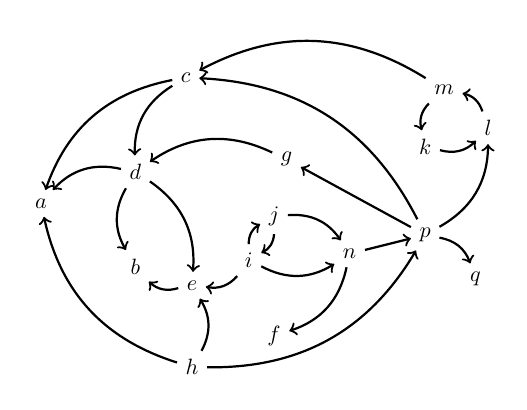
\begin{tikzpicture}[every node/.style={circle, draw, scale=1}, scale=0.8]
  \tikzset{every node/.style={scale=0.8, very thick}} 
  \node (a) at (-0.5, 0.0) {$a$};
  \node (b) at (1.0, -1.0) {$b$};
  \node (c) at (1.8, 2.0) {$c$};
  \node (d) at (1.0, 0.5) {$d$};
  \node (e) at (1.9, -1.3) {$e$};
  \node (f) at (3.2, -2.1) {$f$};
  \node (g) at (3.4, 0.7) {$g$};
  \node (h) at (1.9, -2.6) {$h$};
  \node (i) at (2.8, -0.9) {$i$};
  \node (j) at (3.2, -0.2) {$j$};
  \node (k) at (5.6, 0.9) {$k$};
  \node (l) at (6.6, 1.2) {$l$};
  \node (m) at (5.9, 1.8) {$m$};
  \node (n) at (4.4, -0.8) {$n$};
  \node (p) at (5.6, -0.5) {$p$};
  \node (q) at (6.4, -1.2) {$q$};
  
  
  % top level
  \tikzset{every node/.style={solid}}; 
  \tikzset{mystyle/.style={->,thick}};  
  \path (c) edge [mystyle,bend right] node {} (a);
  \path (c) edge [mystyle,bend right] node {} (d);
  \path (d) edge [mystyle,bend right] node {} (a);
  \path (d) edge [mystyle,bend right] node {} (b);
  \path (d) edge [mystyle,bend left] node {} (e);
  \path (e) edge [mystyle,bend left] node {} (b);
  \path (g) edge [mystyle,bend right] node {} (d);
  \path (h) edge [mystyle,bend left] node {} (a);
  \path (h) edge [mystyle,bend right] node {} (e);
  \path (h) edge [mystyle,bend right] node {} (p);
  \path (i) edge [mystyle,bend left] node {} (e);
  \path (i) edge [mystyle,bend left] node {} (j);
  \path (i) edge [mystyle,bend right] node {} (n);
  \path (j) edge [mystyle,bend left] node {} (i);
  \path (j) edge [mystyle,bend left] node {} (n);
  \path (k) edge [mystyle,bend right] node {} (l);
  \path (l) edge [mystyle,bend right] node {} (m);
  \path (m) edge [mystyle,bend right] node {} (k);
  \path (m) edge [mystyle,bend right] node {} (c);
  \path (n) edge [mystyle,bend left] node {} (f);
  \path (n) edge [mystyle] node {} (p);
  \path (p) edge [mystyle] node {} (g);
  \path (p) edge [mystyle,bend right] node {} (c);
  \path (p) edge [mystyle,bend right] node {} (l);
  \path (p) edge [mystyle,bend left] node {} (q);
\end{tikzpicture}

    }
    \caption{2nd agent}
    \label{fig:full-AF2}
  \end{minipage}
\end{figure}

\subsection{Take 1}
$\langle b, g, h \rangle$ is a successful argument against $\langle d, e \rangle$. 
$$\ddia b \ddia d \ddia g \ddia e \ddia h \cdia (b \wedge g \wedge h)$$
We are not trying to \emph{defend} some given position/set of arguments, but we're rather interested in whether there is some line of arguments which supports $b$ (say credulously). So we check the formula $\ddia b \ddia d \ddia g \ddia e \ddia h \cdia b$. The AF is progressively constructed as shown in Table \ref{tbl:dynamism-1}. For this example, the single agent and multi-agent cases will agree (the evolution in the multi-agent case will be identical because the two agents agree on the edges between the topical arguments.) However, from this point on, interesting things might happen! 

\begin{table}[ht]
  \centering
  \begin{tabular}{l|c|r}
    $\ddia b$ & 
      \begin{tikzpicture}[every node/.style={circle, draw, scale=1}, scale=0.8]
        \tikzset{every node/.style={scale=0.8, very thick}} 
        \node (b) at (1.0, -1.0) {$b$};
      \end{tikzpicture} & \{\{b\}\}  \\ \hline

      $\ddia b \ddia d$ & 
      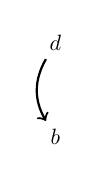
\begin{tikzpicture}[every node/.style={circle, draw, scale=1}, scale=0.8]
        \tikzset{every node/.style={scale=0.8, very thick}} 
        \node (b) at (1.0, -1.0) {$b$};
        \node (d) at (1.0, 0.5) {$d$};
        % top level
        \tikzset{every node/.style={solid}}; 
        \tikzset{mystyle/.style={->,thick}};  
        \path (d) edge [mystyle,bend right] node {} (b);
      \end{tikzpicture} & $\{\{d\}\}$ \\ \hline

      $\ddia b \ddia d \ddia g $ & 
      \begin{tikzpicture}[every node/.style={circle, draw, scale=1}, scale=0.8]
        \tikzset{every node/.style={scale=0.8, very thick}} 
        \node (b) at (1.0, -1.0) {$b$};
        \node (d) at (1.0, 0.5) {$d$};
        \node (g) at (3.4, 0.7) {$g$};
        % top level
        \tikzset{every node/.style={solid}}; 
        \tikzset{mystyle/.style={->,thick}};  
        \path (d) edge [mystyle,bend right] node {} (b);
        \path (g) edge [mystyle,bend right] node {} (d);
      \end{tikzpicture} & $\{\{b, g\}\}$ \\ \hline

      $\ddia b \ddia d \ddia g \ddia e $ & 
      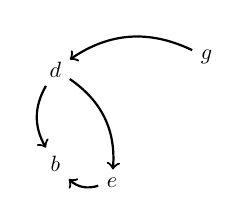
\begin{tikzpicture}[every node/.style={circle, draw, scale=1}, scale=0.8]
        \tikzset{every node/.style={scale=0.8, very thick}} 
        \node (b) at (1.0, -1.0) {$b$};
        \node (d) at (1.0, 0.5) {$d$};
        \node (e) at (1.9, -1.3) {$e$};
        \node (g) at (3.4, 0.7) {$g$};
        % top level
        \tikzset{every node/.style={solid}}; 
        \tikzset{mystyle/.style={->,thick}};  
        \path (d) edge [mystyle,bend right] node {} (b);
        \path (d) edge [mystyle,bend left] node {} (e);
        \path (e) edge [mystyle,bend left] node {} (b);
        \path (g) edge [mystyle,bend right] node {} (d);
      \end{tikzpicture} & $\{ \{e, g\}\}$\\ \hline

      $\ddia b \ddia d \ddia g \ddia e \ddia h$ & 
      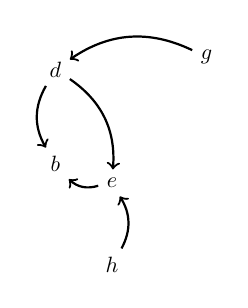
\begin{tikzpicture}[every node/.style={circle, draw, scale=1}, scale=0.8]
        \tikzset{every node/.style={scale=0.8, very thick}} 
        \node (b) at (1.0, -1.0) {$b$};
        \node (d) at (1.0, 0.5) {$d$};
        \node (e) at (1.9, -1.3) {$e$};
        \node (g) at (3.4, 0.7) {$g$};
        \node (h) at (1.9, -2.6) {$h$};
        % top level
        \tikzset{every node/.style={solid}}; 
        \tikzset{mystyle/.style={->,thick}};  
        \path (d) edge [mystyle,bend right] node {} (b);
        \path (d) edge [mystyle,bend left] node {} (e);
        \path (e) edge [mystyle,bend left] node {} (b);
        \path (g) edge [mystyle,bend right] node {} (d);
        \path (h) edge [mystyle,bend right] node {} (e);
      \end{tikzpicture} & $\{ \{b, g, h\}\}$ \\
  \end{tabular}

  \caption{Simple (single-agent/deterministic) ``argument''}
  \label{tbl:dynamism-1}
\end{table}

In the next instance we might try putting forth $q$. This argument would attack $h$ according to agent $2$, but create an isolated pocket in agent $1$'s view, hence we have two cases when evaluating the case $\ddia b \ddia d \ddia g \ddia e \ddia h \ddia q$ as we illustrate in Figure \ref{tbl:dynamism-3}.
%% \begin{table}[ht]
%%   \centering
%%   \begin{tabular}{c|c}
%%     \begin{tikzpicture}[every node/.style={circle, draw, scale=1}, scale=0.8]
%%       \tikzset{every node/.style={scale=0.8, very thick}} 
%%       \node (b) at (1.0, -1.0) {$b$};
%%       \node (d) at (1.0, 0.5) {$d$};
%%       \node (e) at (1.9, -1.3) {$e$};
%%       \node (g) at (3.4, 0.7) {$g$};
%%       \node (h) at (1.9, -2.6) {$h$};
%%       \node (q) at (6.4, -1.2) {$q$};
%%         % top level
%%       \tikzset{every node/.style={solid}}; 
%%       \tikzset{mystyle/.style={->,thick}};  
%%       \path (d) edge [mystyle,bend right] node {} (b);
%%       \path (d) edge [mystyle,bend left] node {} (e);
%%       \path (e) edge [mystyle,bend left] node {} (b);
%%       \path (g) edge [mystyle,bend right] node {} (d);
%%       \path (h) edge [mystyle,bend right] node {} (e);
%%     \end{tikzpicture} &
%%     \begin{tikzpicture}[every node/.style={circle, draw, scale=1}, scale=0.8]
%%       \tikzset{every node/.style={scale=0.8, very thick}} 
%%       \node (b) at (1.0, -1.0) {$b$};
%%       \node (d) at (1.0, 0.5) {$d$};
%%       \node (e) at (1.9, -1.3) {$e$};
%%       \node (g) at (3.4, 0.7) {$g$};
%%       \node (h) at (1.9, -2.6) {$h$};
%%       \node (q) at (6.4, -1.2) {$q$};
%%       % top level
%%       \tikzset{every node/.style={solid}}; 
%%       \tikzset{mystyle/.style={->,thick}};  
%%       \path (d) edge [mystyle,bend right] node {} (b);
%%       \path (d) edge [mystyle,bend left] node {} (e);
%%       \path (e) edge [mystyle,bend left] node {} (b);
%%       \path (g) edge [mystyle,bend right] node {} (d);
%%       \path (h) edge [mystyle,bend right] node {} (e);
%%       \path (q) edge [mystyle,bend left] node {} (h);
%%     \end{tikzpicture} \\ \hline
%% $\{\{b, g,h,q\}\}$ & $ \{ \{e, g, q\}\}$ \\
%%   \end{tabular}
  
%%   \caption{$\ddia b \ddia d \ddia g \ddia e \ddia h \ddia q$}
%%   \label{tbl:dynamism-2}
%% \end{table}

So, indeed, we see that \emph{there is some} was of putting forth $q$ at this stage such that $b$ is accepted (even skeptically), and another way which yields $b$ not being acceptable at all. Can we now attack $q$ with, say $p$? No. Not successfully. Since both agents agree that $g$ attacks $p$ we are required to include this edge when putting forth $p$. So in these two cases we obtain the situations depicted in Table \ref{tbl:dynamism-3}.

\begin{figure}[ht]
  \centering
  \def\svgwidth{\textwidth}
  \begin{tiny}
    \input{img/graph-tree.pdf_tex}
  \end{tiny}
  \caption{$\ddia b \ddia d \ddia g \ddia e \ddia h \ddia q \ddia p$}
  \label{tbl:dynamism-3}
\end{figure}

Observe that we've now introduced, in one of the resulting graphs a pattern which doesn't occur in any of the agents' AFs. See for example the 3-cycle over $p$, $q$ and $h$! 

Let us now examine the possible deliberative scenarios surrounding the argument $e$. We will state $e$ to have it tested $\ddia e$. We then try to counter it and see if it survives deliberation. Obviously, $e$ can be countered, $\ddia e \adia \neg \cdia e$. However, what we want to find out is whether it \emph{can} survive such a process, i.e., whether $\ddia e \abox \adia \cdia e$. Consider every argument $x$ which could have, some of them will leave $e$ unattacked, in which case we can simply restate $e$ for our $\adia$-step and we'll have $\cdia e$. Otherwise, if the argument $x$ attacks $e$ it is one of $d$, $i$ and $h$, but each of these can in turn be rebutted at the $\adia$-step by, respectively, $c$ and $g$, $j$, and $q$. Observe that if we have to rebut $h$ with $q$ we're relying on the fact that one of the agents accepts that $q \longrightarrow h$. 


%% \section{The Logic (2)}
%% In this section we generalize our logic and characterize some classes of deliberative models which we argue are of intereset in themselves, and furthermore, illustrates the framework we are proposing. We remove from the language the ability to refer to explicit arguments in the logic, but introduce a new connective. 

%% \begin{definition}The language $\langb$ is given by the following BNF
%% $$\phi \quad ::= \quad \cdia \alpha ~|~ \neg \phi ~|~ \phi \wedge \phi ~|~ \adia \phi ~|~ \adiastar \phi $$
%% where $\alpha \in \lblack$.
%% \end{definition}


%% \subsection{Right-or-wrong}
%% The class of right-or-wrong is a set of models, where the proponents separate in clear parties. Suppose we have $n$ agents and $m \leq n$ parties. We separate each argument in one of $m$ partitions $\Pi_m$ partitions $\Pi$, such that if agent $i$ is in party $j$ then agent $i$ has no arrows into $\Pi_m$. This, obviously, permits that an agent belongs to more than one party, but this is not relevant for our argument so we'll just assume for the time being that they all belong to some party. I.e., 

%% \begin{definition}A $m$-row-model is a model $V = \langle \agents, \Pi, (V_a)_{(a \in \agents)} \rangle$ such that
%% \begin{itemize}
%% \item there is a partitioning of arguments $m^\Pi$ and agents $\rho : n \to m$, which satisfies 
%%   $$\rho(i) = j \Rightarrow \forall (x,y) \in V_i \Rightarrow y \notin \Pi_j$$
%% \end{itemize}
%% \end{definition}


%% \subsection{Everything-is-true (occationally)}
%% The class of Everything-is-true-(occationally)-models is the collection of models where, for every argument $p \in \Pi$, there is some state of affairs which makes $p$ true in some extension. 

%% \begin{definition} An eito-model is a model $V = \langle \agents, \Pi, (V_a)_{(a \in \agents)} \rangle$ such that
%% \begin{itemize}
%% \item for every argument $p \in \Pi$, 
%% $$ \mm, (\emptyset, \emptyset) \models \adiastar \cdia p$$
%% \end{itemize}
%% \end{definition}

%% Perhaps that's not what eito-models look like. Perhaps they need to look like
%% \begin{itemize}
%% \item for every argument $p \in \Pi$, for every reachable point $q$ 
%% $$ \mm, q \models \adiastar \cdia p$$
%% \end{itemize}
%% \truls{... but maybe we should talk about it...}


\section{Conclusion and Future work}
\begin{itemize}
\item Restrict states to  $\subseteq_{\text{fin}}$.
\item Reflect on limits, infinite sequences in our tree structures, etc...
\item Discuss the white diamond as the iteration of the union of all programs; say it's impossible in DPL, but we want to do it anyway.
\end{itemize}

\bibliographystyle{abbrv}
\bibliography{cites, morecites}
\end{document}


%% Big (original) graph
%% \newpage
%% \begin{figure}[ht]
%% \centering
%% \input{img/big-graph.pdf_tex}
%% \caption{Inkscape to \LaTeX -test}
%% \end{figure}
